\documentclass[]{tufte-book}

% ams
\usepackage{amssymb,amsmath}

\usepackage{ifxetex,ifluatex}
\usepackage{fixltx2e} % provides \textsubscript
\ifnum 0\ifxetex 1\fi\ifluatex 1\fi=0 % if pdftex
  \usepackage[T1]{fontenc}
  \usepackage[utf8]{inputenc}
\else % if luatex or xelatex
  \makeatletter
  \@ifpackageloaded{fontspec}{}{\usepackage{fontspec}}
  \makeatother
  \defaultfontfeatures{Ligatures=TeX,Scale=MatchLowercase}
  \makeatletter
  \@ifpackageloaded{soul}{
     \renewcommand\allcapsspacing[1]{{\addfontfeature{LetterSpace=15}#1}}
     \renewcommand\smallcapsspacing[1]{{\addfontfeature{LetterSpace=10}#1}}
   }{}
  \makeatother

\fi

% graphix
\usepackage{graphicx}
\setkeys{Gin}{width=\linewidth,totalheight=\textheight,keepaspectratio}

% booktabs
\usepackage{booktabs}

% url
\usepackage{url}

% hyperref
\usepackage{hyperref}

% units.
\usepackage{units}


\setcounter{secnumdepth}{2}

% citations
\usepackage{natbib}
\bibliographystyle{plainnat}

% pandoc syntax highlighting

% longtable
\usepackage{longtable,booktabs}

% multiplecol
\usepackage{multicol}

% strikeout
\usepackage[normalem]{ulem}

% morefloats
\usepackage{morefloats}


% tightlist macro required by pandoc >= 1.14
\providecommand{\tightlist}{%
  \setlength{\itemsep}{0pt}\setlength{\parskip}{0pt}}

% title / author / date
\title{Atlas of Bacterial and Archaeal Cell Structure}
\author{Catherine M. Oikonomou and Grant J. Jensen}
\date{2020-10-06}

\usepackage{booktabs}
\usepackage{amsthm}
\makeatletter
\def\thm@space@setup{%
  \thm@preskip=8pt plus 2pt minus 4pt
  \thm@postskip=\thm@preskip
}
\makeatother

\begin{document}

\maketitle



{
\setcounter{tocdepth}{1}
\tableofcontents
}

\chapter*{Introduction}\label{introduction}
\addcontentsline{toc}{chapter}{Introduction}

\begin{quote}
``It is very easy to answer many of these fundamental biological
questions; you just \emph{look at the thing!}'' - Richard Feynman
\citep{feynman1960}
\end{quote}

\chapter{Introduction}\label{intro}

\section{Markdown syntax}\label{markdown-syntax}

Markdown is a simple text-based way of formatting documents. There are
many flavors of markdown, we'll start with standard markdown and then
add some specific rmarkdown information. Let's look at some other
basics:

\begin{itemize}
\tightlist
\item
  You can put text into \emph{italics} and \textbf{bold} using * or **
\item
  To create headings, put one or more \# symbols at the beginning of a
  line, followed by a space. One \# is for a level one header, \#\# for
  a level two header, etc.
\item
  To make bullet lists (such as this one), just start lines with a -;
  you can get additional levels by starting a line a couple of spaces or
  a tab in. Numbered lists work the same way using 1. 2. 3.
\end{itemize}

\texttt{-\ Topic\ 1\ \ \ \ \ -\ Topic\ 2\ \ \ \ \ \ \ -\ Topic\ 3\ \ \ \ \ \ \ -\ Topic\ 3a}
- To cite code (including markdown syntax as above) use ` on both sides
for short bits and ``` in a separate line above and below larger
codeblocks. - Quote text using \textgreater{} at the beginning of the
line (maybe you remember this from old e-mail programs?)

\texttt{\textgreater{}\ This\ is\ a\ Quote}

\begin{itemize}
\tightlist
\item
  A link is set putting the text that you want to highlight in square
  brackets followed by the link in round brackets. Don't forget to
  include \url{http://} or \url{https://} at the beginning of the link
\end{itemize}

\texttt{{[}This\ is\ a\ link{]}(http://www.example.com)} - You can find
more markdown formatting options
\href{https://guides.github.com/features/mastering-markdown/}{here}.
Note that markdown comes in different dialects, referred to as
``flavors''. We are mainly going to be using elements that are part of a
consensus referred to as \href{http://commonmark.org/}{Common Markdown},
though you can use any other components of the github flavored markdown
linked above.

\section{Bookdown Specific Features}\label{bookdown-specific-features}

You can label chapter and section titles using \texttt{\{\#label\}}
after them, e.g., we can reference Chapter \ref{intro}. If you do not
manually label them, there will be automatic labels anyway, e.g.,
Chapter \ref{methods}.

Figures and tables with captions will be placed in \texttt{figure} and
\texttt{table} environments, respectively.

\begin{figure}

{\centering 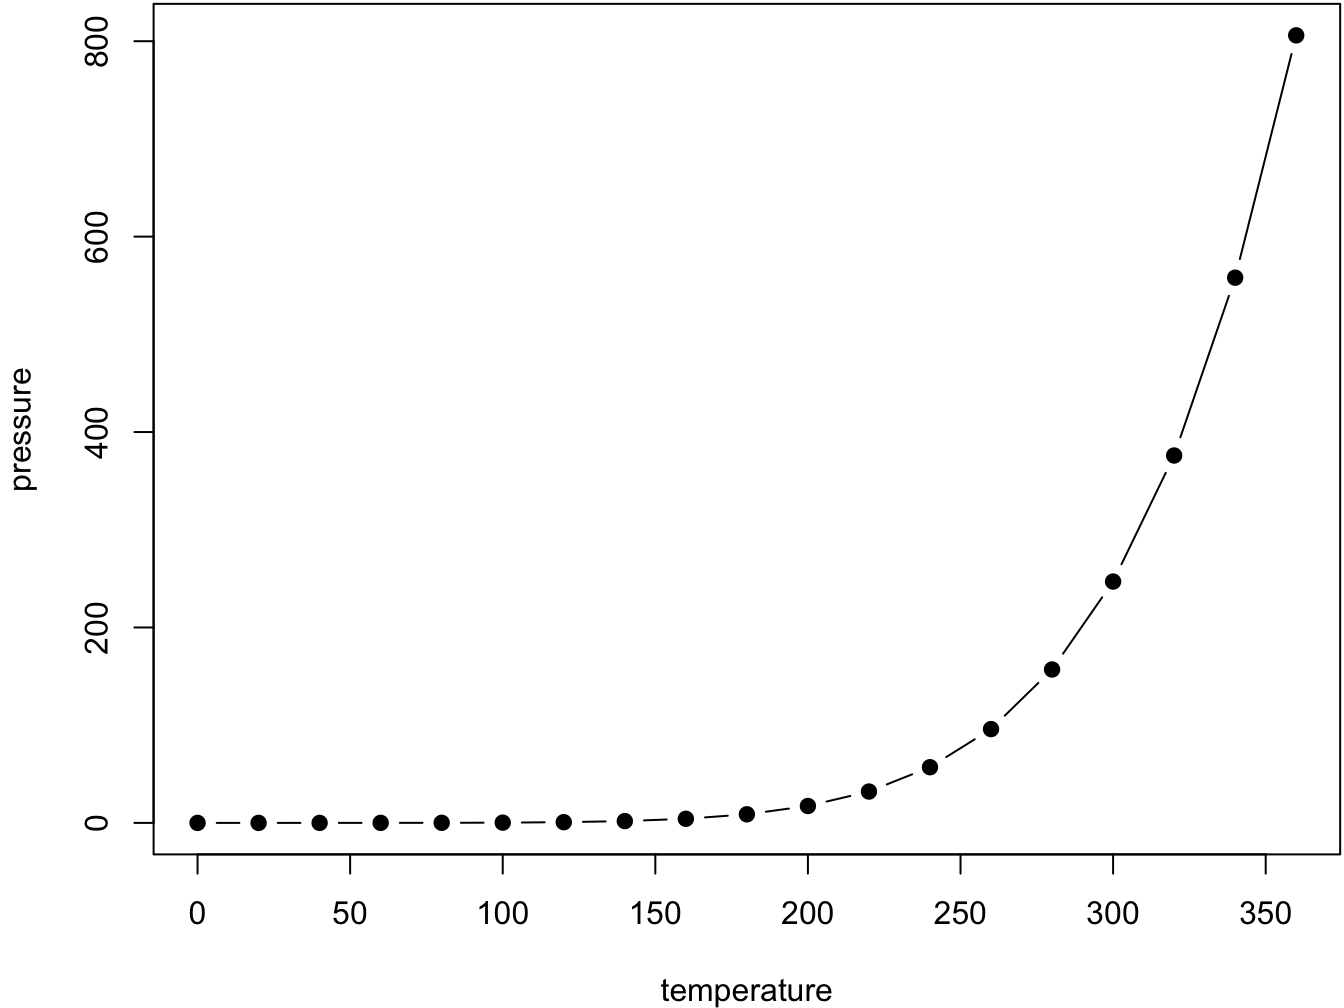
\includegraphics[width=0.8\linewidth]{book_files/figure-latex/nice-fig-1} 

}

\caption[Here is a nice figure!]{Here is a nice figure!}\label{fig:nice-fig}
\end{figure}

Reference a figure by its code chunk label with the \texttt{fig:}
prefix, e.g., see Figure \ref{fig:nice-fig}. Similarly, you can
reference tables generated from \texttt{knitr::kable()}, e.g., see Table
\ref{tab:nice-tab}.

\begin{table}

\caption{\label{tab:nice-tab}Here is a nice table!}
\centering
\begin{tabular}[t]{rrrrl}
\toprule
Sepal.Length & Sepal.Width & Petal.Length & Petal.Width & Species\\
\midrule
5.1 & 3.5 & 1.4 & 0.2 & setosa\\
4.9 & 3.0 & 1.4 & 0.2 & setosa\\
4.7 & 3.2 & 1.3 & 0.2 & setosa\\
4.6 & 3.1 & 1.5 & 0.2 & setosa\\
5.0 & 3.6 & 1.4 & 0.2 & setosa\\
\addlinespace
5.4 & 3.9 & 1.7 & 0.4 & setosa\\
4.6 & 3.4 & 1.4 & 0.3 & setosa\\
5.0 & 3.4 & 1.5 & 0.2 & setosa\\
4.4 & 2.9 & 1.4 & 0.2 & setosa\\
4.9 & 3.1 & 1.5 & 0.1 & setosa\\
\addlinespace
5.4 & 3.7 & 1.5 & 0.2 & setosa\\
4.8 & 3.4 & 1.6 & 0.2 & setosa\\
4.8 & 3.0 & 1.4 & 0.1 & setosa\\
4.3 & 3.0 & 1.1 & 0.1 & setosa\\
5.8 & 4.0 & 1.2 & 0.2 & setosa\\
\addlinespace
5.7 & 4.4 & 1.5 & 0.4 & setosa\\
5.4 & 3.9 & 1.3 & 0.4 & setosa\\
5.1 & 3.5 & 1.4 & 0.3 & setosa\\
5.7 & 3.8 & 1.7 & 0.3 & setosa\\
5.1 & 3.8 & 1.5 & 0.3 & setosa\\
\bottomrule
\end{tabular}
\end{table}

You can write citations, too. For example, we are using the
\textbf{bookdown} package \citep{R-bookdown} in this sample book, which
was built on top of R Markdown and \textbf{knitr} \citep{xie2015}.

\chapter{Cells}\label{cells}

\begin{quote}
``It is not a simple life to be a single cell, although I have no right
to say so, having been a single cell so long ago myself that I have no
memory at all of that stage of my life.'' - Lewis Thomas
\citep{thomas1990}
\end{quote}

\section{Membrane}\label{membrane}

The fundamental unit of life is the \textbf{cell}--a contained
self-replicating assembly. For many species, including all bacteria and
archaea, the organism consists of a single cell. And for nearly all
species, no matter how many cells an organism eventually contains
(probably around 10 trillion in your case), it started life as a single
cell. The details vary, but every cell on Earth is the same at heart--a
DNA-based replicating machine built from just four macromolecules:
nucleic acids, proteins, lipids and carbohydrates. In the environment,
molecules interact rarely and randomly. Bringing them together enables
the reproducible reactions required for life. So no matter what the
first self-replicating molecules were (likely ribonucleic acid, or RNA),
they were not a cell until they acquired a container.

How would you build a container for a cell? You would probably want a
flexible material that allowed you to sort specific molecules from the
environment. Evolution agrees. All cells are enclosed by a selectively
permeable \textbf{membrane}, made of lipids and proteins
\protect\hyperlink{Lipid_bilayer}{Schematic: Lipid bilayer}, that allows
them to differentiate their contents from the environment. The chemical
properties of lipids make membranes impermeable to ions and large or
hydrophilic molecules (but not to water). Cells take advantage of this
property to establish an ion gradient across the membrane, using a chain
of electron-carrying proteins in the membrane to pump protons out of the
cell. Protein complexes in the membrane called ATP synthases use the
resulting ion potential to generate energy that is chemically stored in
ATP, the energetic currency of the cell. For this reason, we say that
the membrane is ``energized.'' Holes in the membrane allow the ion
gradient to equilibrate, destroying the cell's means of generating
energy, and thus its life.

Now your cell has a clearly delineated exterior and interior. The
interior is called the \textbf{cytoplasm} (``cell substance,'' from the
Latin for something molded, in this case by the membrane). Almost all
archaea and many bacteria, like these \emph{Mycoplasma genitalium}
cells, are \textbf{monoderms} (``single skin''). This means that their
cytoplasm is enclosed by a single membrane. At this resolution, the
membrane looks like a single dark line, but remember that it is really a
bilayer, as you will be able to see in some later examples. The
cytoplasm contains the many macromolecules that carry out the various
functions of the cell's metabolism. The most prominent are the ribosomes
which produce new proteins \protect\hyperlink{Ribosome}{Schematic:
Ribosome}.

Other structures you see in this cell function in motility and will be
explained in Chapter 6. Remember that tomograms show cells in their
entirety, so the example we choose to illustrate one feature will likely
highlight others as well. For now, focus on the feature being discussed.
Later, when you have learned about other features, you may want to see
additional examples of them. Then you can use the {[}Feature Index{]} to
find them. To help orient you, feature labels in movies are color-coded
according to the chapter in which they are discussed.





\begin{figure}
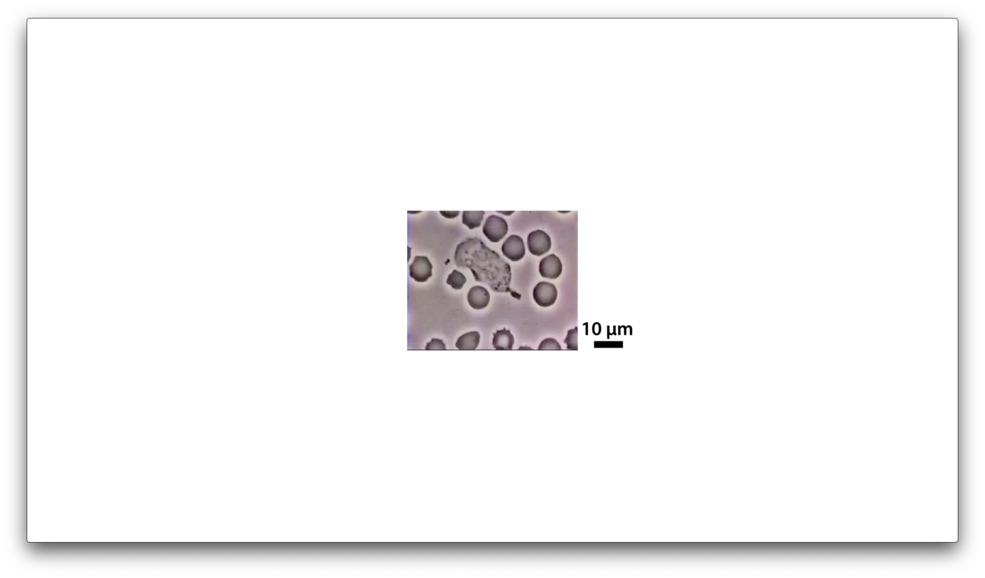
\includegraphics{movie_stills/1_1} \caption[\protect\hyperlink{tree}{Staphylococcus aureus} Collected by:
\protect\hyperlink{david_rogers}{David Rogers} Movie DOI:
\href{https://doi.org/10.22002/D1.1463}{10.22002/D1.1463}]{\protect\hyperlink{tree}{Staphylococcus aureus} Collected by:
\protect\hyperlink{david_rogers}{David Rogers} Movie DOI:
\href{https://doi.org/10.22002/D1.1463}{10.22002/D1.1463}}\label{fig:1-1}
\end{figure}

\begin{figure}
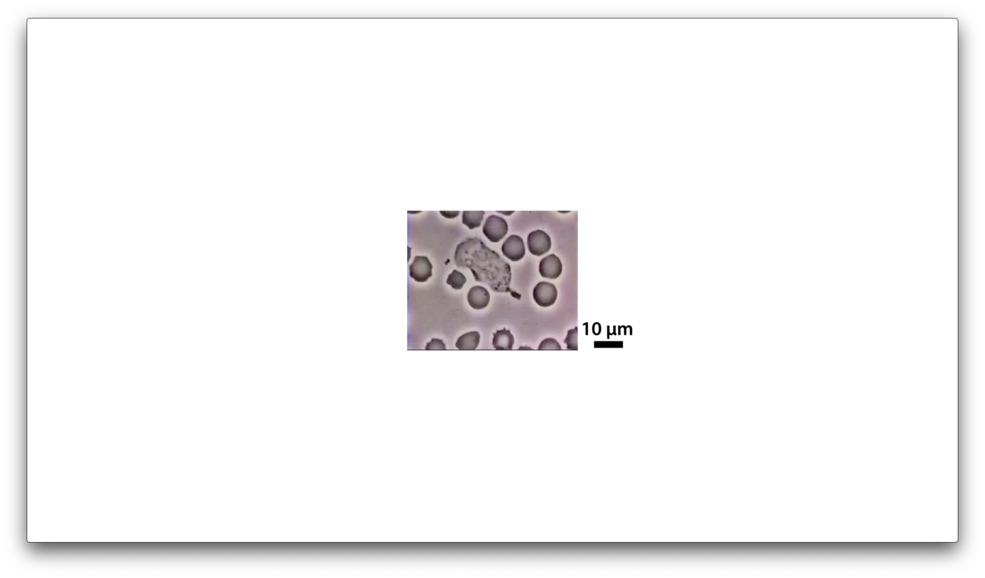
\includegraphics{movie_stills/1_1} \caption[(ref:1-1-embed)]{(ref:1-1-embed)}\label{fig:1-1-embed}
\end{figure}

\subsection*{Schematic: Bactofilin}\label{Bactofilin}
\addcontentsline{toc}{subsection}{Schematic: Bactofilin}

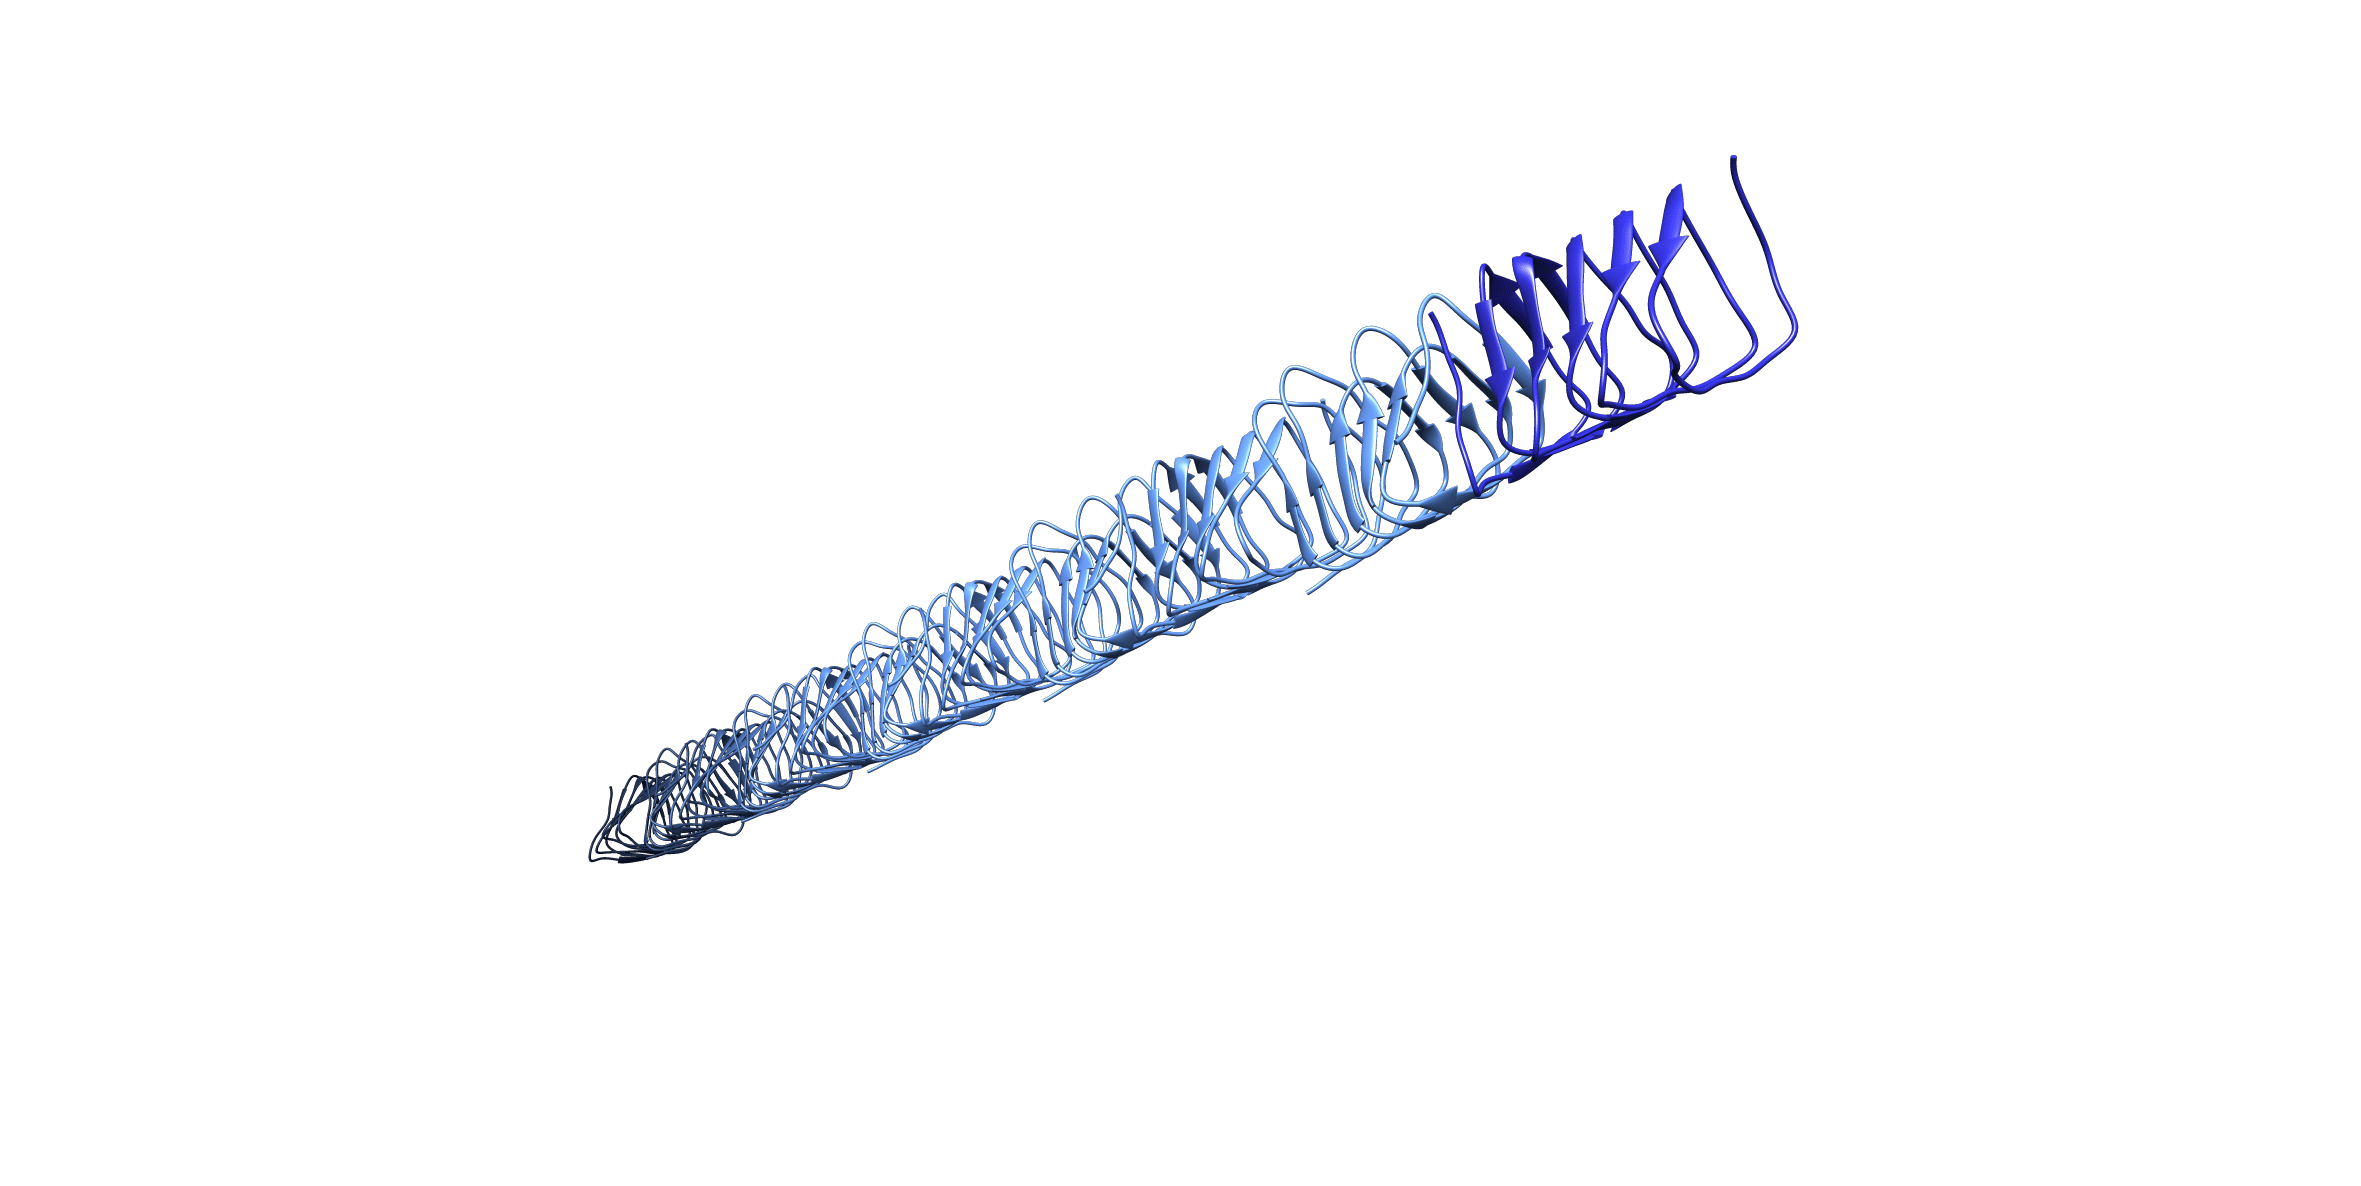
\includegraphics{img/3_6_1}

\href{http://rcsb.org/structure/6RIB}{\emph{PDB: 6RIB}} Bactofilins are
found in many species of bacteria and archaea, suggesting that they
perform diverse (and currently unknown) functions. They polymerize into
very stable filaments with a triangular beta-helical structure, like
this one from \emph{Thermus thermophilus} \citep{deng2019}. Bactofilin
filaments lack two hallmarks of actin- and tubulin-based cytoskeletal
elements: polarity and dynamic assembly/disassembly. In this way, they
are similar to intermediate filaments in eukaryotic cytoskeletons.

\subsection*{Further Reading}\label{further-reading}
\addcontentsline{toc}{subsection}{Further Reading}

Errington (2013). \emph{L-form bacteria, cell walls and the origins of
life} \citep{errington2013}.

Ptacin and Shapiro (2013). \emph{Chromosome architecture is a key
element of bacterial cellular organization} \citep{ptacin2013}.

Sleytr and Beveridge (1999). \emph{Bacterial S-layers}
\citep{sleytr1999}.

Strahl and Errington (2017). \emph{Bacterial membranes: Structure,
domains, and function} \citep{strahl2017}.

\bibliography{AtlasBibTeX.bib}



\end{document}
